\section{Database caching}

WordPress was programmed with the support of database caching in mind. Core functions and methods querying the database (such as get\_option, get\_posts and others) use WordPress Object Cache API \cite{WP:Object-Cache-API} on the background. \\

The default Object Cache API caches the database queries and results in a PHP array, thus only for a duration of the script execution (one request). On one hand, this mechanism is useful in templates, where the same information about the site is retrieved multiple times (for example get\_bloginfo function). On the other hand, when many users visiting our site request the same page, the same database queries have to be made unnecessarily multiple times. \\

If we need to store the database cache persistently, we can use an in-memory database. "An in-memory database is a database management system that primarily relies on main memory for computer data storage. It is contrasted with database management systems that employ a disk storage mechanism. Main memory databases are faster than disk-optimized databases since the internal optimization algorithms are simpler and execute fewer CPU instructions. Accessing data in memory eliminates seek time when querying the data, which provides faster and more predictable performance than disk." \cite{Wiki:in-memory-database}\\

The two most popular in-memory databases in the WordPress ecosystem are Memcached and Redis. In our work we have chosen to work with Redis as it is modern, well-supported and having all the features of Memcached. \cite{SO:Redis-vs-Memcached} In order for WordPress Object Cache API to use Redis for database caching, we need to install Redis server and Redis PHP connector (driver). We have prepared an Ansible playbook which downloads a PHP driver for Redis and installs it into the currently installed WordPress site (whether basic or advanced). Within your command line, navigate to the wordpress-ansible directory and run the "wordpress\_redis\_db\_cache.yml" Ansible playbook:

\begin{lstlisting}
ansible-playbook -i hosts wordpress\_redis\_db\_cache.yml
\end{lstlisting}

Analogous to how we benchmarked the web-serving software in the previous section, we configured a Loader.io test and performed several load tests for the site with Redis database caching enabled. Suprisingly, resulting charts did not show any noticeable improvements \cite{Loader.io:nginx_hhvm_redis} over the other tests. Contemplating over this issue, we think that the database on our testing server is not a bottleneck. However, as this has not been proved yet, it might be a subject of a future work.

\section{Page caching} \label{page-caching}

To improve the performance even more, we can actually cache the result of the PHP processing of our site. We can save the resulting HTML file on a disk or to a RAM memory and when the next request arrives, just output the cached page. Full page caching can be done on several abstraction levels. The easiest one to set up is to have a WordPress plugin construct a static HTML cache of each requested web page on your site and store it as a flat file on your server disk drive. The problem with this approach is that there still has to be some kind of routing done on the PHP level as Nginx doesn't know which file to load on a request. Hard-drive cna also easily become a bottleneck if a lot of concurrent clients are loading the site, thus reading the file.

Better solution is to have the page cache done on a lower level, the Nginx one. Nginx has a fastcgi cache module for exactly this purpose. We can configure Nginx to store the output from PHP processor into the RAM (tmpfs file system). When a new request comes, Nginx checks whether there already is a cached page or not. If it is, it will return it back to the user as a response. If it is not, it will forward the request to the PHP listening on the FastCGI server. When the resulting HTML file gets back to Nginx, it will store it in the page cache on the RAM for later usage.

This process is rather fast, as Nginx is able to respond to thousands of concurrent requests, as seen from the chart below. Nginx uses a tree-like structure to store the data with hashing mechanisms, thus increasing the performance.

In order to revalidate and purge the old data, a Nginx location directive can be added. This directive can then be called from within WordPress to purge the cache if new content was added to our site. There is a handy plugin called Nginx Helper from rtcamp which automatically purges the cache on new post or page addition.

Run nginx-page-cache.yaml playbook to have your VPS server fully configured with Nginx FastCGI page caching.

The downsides of page caching are that if a cached page is updated – just a small part of it — you need to purge it from the cache and re-load it. If a person is logged in WordPress, it's not possible to cache most pages because they are customized for the particular user. Solutions such as CacheBuddy are specially made for this purpose.

Better than W3 Total Cache page caching because it goes directly into RAM, can skip caching if cookie is present or specific location, relying on nginx caching mechanisms, fast, can be purged automatically on new post/page, etc.

\begin{figure}[H]
\begin{center}
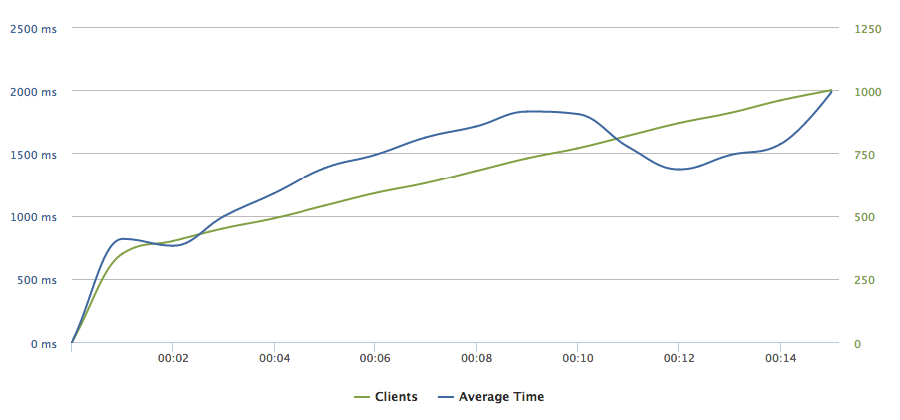
\includegraphics[scale=0.5]{figures/Nginx_FastCGI_caching.png}
\caption{Nginx with FastCGI caching: clients versus average response time}
\label{fig:nginx_fastcgi_caching}
\end{center}
\end{figure}

\begin{figure}[H]
\begin{center}
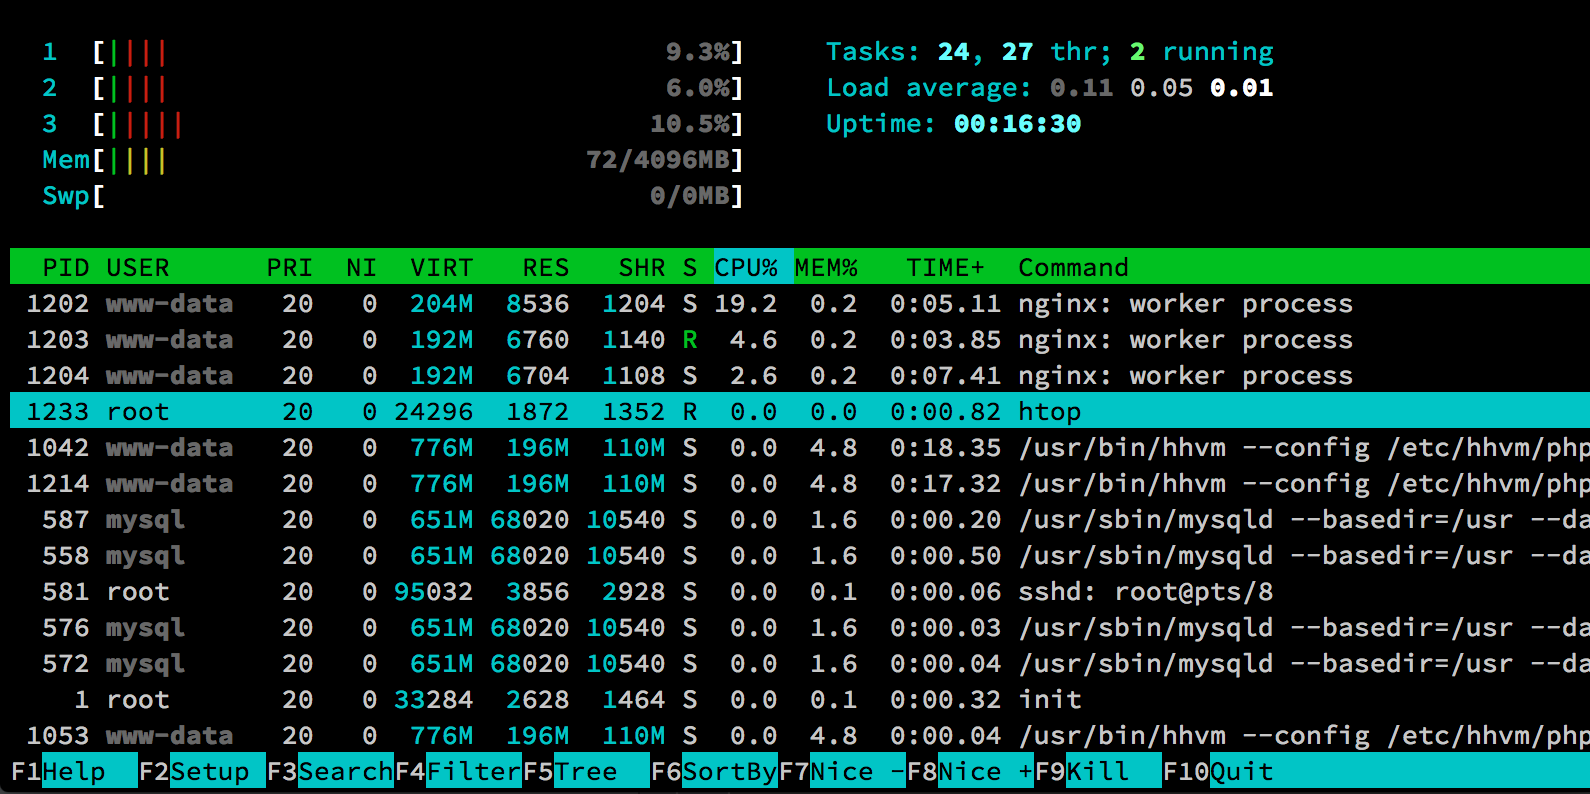
\includegraphics[scale=0.5]{figures/Nginx_FastCGI_caching_9s.png}
\caption{Nginx with FastCGI caching: Htop process viewer 9 seconds into test}
\label{fig:nginx_fastcgi_caching}
\end{center}
\end{figure}

\section{Browser caching}

Browser caching is the process of storing data in the client's browser memory. If we store the resources (CSS, JS, images and fonts) and HTML pages in the client's browser cache, the browser doesn't have to load the resources from our servers, therefore saving time and bandwidth and server processing power.

The main disadvantage of browser caching is that if addition to the resources were added or content changed, we need to revalidate the cache somehow. As the cached resources are not loaded from our server, we need to do it some other way. The preferred way to purge browser cache is to rename the resources so the browser will see them as new files which it has to load again.

To set caching, we need to specify caching options and expiration date as headers when serving files from Nginx. 

Ansible playbook..
